\documentclass[a4paper,10pt]{article}
\usepackage[margin=2.5cm]{geometry}
\usepackage[utf8]{inputenc}
\usepackage[colorlinks=true,urlcolor=blue]{hyperref}
\usepackage{amsmath}
\usepackage{graphicx}
\usepackage{float}
\usepackage{caption}
\usepackage{xcolor}
\usepackage{booktabs}

\usepackage{listings} %Alternative to minted
\definecolor{codegreen}{rgb}{0,0.6,0}
\definecolor{codegray}{rgb}{0.5,0.5,0.5}
\definecolor{codepurple}{rgb}{0.58,0,0.82}
\definecolor{backcolour}{rgb}{0.95,0.95,0.92}
 
\lstdefinestyle{mystyle}{
    backgroundcolor=\color{backcolour},   
    commentstyle=\color{codegreen},
    keywordstyle=\color{magenta},
    numberstyle=\tiny\color{codegray},
    stringstyle=\color{codepurple},
    basicstyle=\footnotesize,
    breakatwhitespace=false,         
    breaklines=true,                 
    captionpos=b,                    
    keepspaces=true,                 
    numbers=left,                    
    numbersep=5pt,                  
    showspaces=false,                
    showstringspaces=false,
    showtabs=false,                  
    tabsize=2
}

\lstset{style=mystyle}
\setlength{\parindent}{0em}
\setlength{\parskip}{1em}

\title{\textbf{Deep Learning for Image Analysis} 
\\ DL4IA -- Report for Assignment 2}
\author{Student Linus Falk}
\date{\today}

\begin{document}
\lstset{language=Python}
\maketitle

\section{Introduction}
Second assignment in the course Deep learning for image analysis

\section{Mathematical exercises}
Given the linear model and multinomial cross-entropy loss:

    \begin{equation}
        z_i = \textbf{W}\textbf{x}_{i} + \textbf{b}, \quad i = 1,2,\ldots,n
    \end{equation}

    \begin{equation}
        L_i = \ln \left( \sum_{l=1}^{M} e^{z_{il}}\right) - \sum_{m=1}^{M}\overset{\sim}{y}_{im}z_{im}, \quad J = \frac{1} {n} \sum_{i=1}^{n} L_i  
    \end{equation}

Were $\overset{\sim}{y}_{im}$ is the hot encoding of the true label $y_i$ for data point $i$

\textit{\textbf{Exercise 1.1}}
Derive the expressions for $\frac{\partial J} {\partial b_m} $ and $  \frac{\partial J} {\partial w_{mj}} $ in terms of: $ \frac{\partial J} {\partial z_{im}}, \frac{\partial z_{im}} {\partial b_m}, \frac{\partial z_{im}} {\partial w_{mj}} $:

    \begin{equation}
    \begin{aligned}
        \frac{\partial J} {\partial b_{m}} = \frac{\partial J} {\partial z_{im}}  \frac{\partial z_{im}} {\partial b_{m}}  \\
        \frac{\partial J} {\partial w_{mj}} = \frac{\partial J} {\partial z_{im}}  \frac{\partial z_{im}} {\partial w_{mj}}
    \end{aligned}
    \end{equation}

We start with $\frac{\partial J} {\partial z_{im}} $

    \begin{equation}
    \begin{aligned}
        \frac{\partial J} {\partial z_{im}} = \frac{\partial } {\partial z_{im}} \ln \left( \sum_{l=1}^{M} e^{z_{il}}\right) - \overset{\sim}{y}_{im}z_{im}  = \frac{\partial } {\partial z_{im}} \ln \left( \sum_{l=1}^{M} e^{z_{il}}\right) - \frac{\partial } {\partial z_{im}} \overset{\sim}{y}_{im}z_{im} = \\
        \frac{e^{z_{il}}} {\sum_{l=1}^{M} e^{z_{il}}} - \overset{\sim}{y}_{im} = \hat{y}_{im} - \overset{\sim}{y}_{im}
    \end{aligned}
    \end{equation}

Were we recognize the fraction as the softmax activation function. We then continue with $\frac{\partial z_{im}} {\partial b_{m}}$ and $\frac{\partial z_{im}} {\partial w_{mj}}$ 

    \begin{equation}
    \begin{aligned}
         \frac{\partial z_{im}} {\partial b_{m}} = \frac{\partial} {\partial b_{m}} \textbf{W}_m\textbf{x}_{im} + \textbf{b}_m = 1 \\
         \frac{\partial z_{im}} {\partial w_{mj}} = \frac{\partial} {\partial b_{m}} \textbf{W}_m\textbf{x}_{im} + \textbf{b}_m = \textbf{x}_{im}
    \end{aligned}
    \end{equation}

\section{Code exercises}

\textit{\textbf{Exercise 1.2}}
Using the \textbf{numpy} library in \textbf{Python}, a feed forward neural network was implemented for solving a classification problem. Following functions were implemented: 

\begin{enumerate}
    \item The \emph{initialize\_parameters} function is used to initialize the weights and offsets by method X. The weight are initialized randomly with mean 0 and variance 0.01 to break the symmetry in the network, making sure that all neurons doesn't learn the same function. 

\begin{lstlisting}
class NeuralNetwork:
    def __init__(self, features, learningRate, X_train, Y_train, X_test,Y_test):
        self.features = features
        self.learningRate = learningRate
        self.layers = []
        self.layersIO = []
        self.layerGradients = []
        self.training_history = []
        self.test_history = []
        self.accuracy = []
        self.test_accuracy = []
        self.iterations = []

    def create_layer(self, nodes, activation):
    ''' 
    param arg 1: Number of nodes in layer
    param arg 2: Activation functions for layer

    return : Initializes a layer with weights and bias, IO (input/output) list for keeping track and gradients for backward propagation
    '''
        np.random.seed(42)
        weights = np.random.rand(nodes[1], nodes[0]) *  0.01 
        bias = np.random.rand(nodes[1], 1) * np.sqrt(1 / (nodes[0]))
        self.layers.append([weights, bias, activation]) 
        self.layersIO.append([None, None, None]) # [input, Z, A]
        self.layerGradients.append([None, None, None, None]) #[dZ, dW, dB, dA]
\end{lstlisting}

    \item Activation functions \emph{relu} and \emph{sigmoid}

\begin{lstlisting}
    def sigmoid(self, Z):
        A = 1 / (1 + np.exp(-Z))
        return A

    def relu(self, Z):
        return np.maximum(Z,0)
\end{lstlisting}
    
    \item Forward propagation with \emph{linear\_forward} computing the linear model of the node, \emph{activation\_forward} for computing the activation after the linear computations and \emph{model\_forward} that combine these and compute the forward pass for the whole model. 

\begin{lstlisting}
    def linear_forward(self, layer , input):
    '''
    param arg 1: The layer that will be calculated in forward pass
    param arg 2: The input to the layer that will be calculated in forward pass

    return: Returns the calculated linear forward pass to the layers IO list 
    '''
        Z = np.dot(self.layers[layer][0], input) + self.layers[layer][1]   
        self.layersIO[layer][0] = input #input
        self.layersIO[layer][1] = Z #dotproduct

    def activation_forward(self, layer):
    '''
    param arg 1: the layer to calculate the activation of 

    return: Activation of the calculated linear forward pass of the layer
    '''
        if self.layers[layer][2] == 'relu':
            A = self.relu(self.layersIO[layer][1]) #activation of dotproduct
            self.layersIO[layer][2] = A #save activated dotproduct array

        elif self.layers[layer][2] == 'sigmoid':
            A = self.sigmoid(self.layersIO[layer][1])
            self.layersIO[layer][2] = A
                    
        elif self.layers[layer][2] == 'softmax':
            A = self.softmax(self.layersIO[layer][1])
                self.layersIO[layer][2] = A
      
    def model_forward(self, minibatch_X): 
    '''
    param arg 1: batch for forward pass of the whole model

    return: the updated IO for all layers 
    '''
        self.linear_forward(0, minibatch_X)
        self.activation_forward(0)
        for i in range(1,len(self.layers),1):
            self.linear_forward(i, self.layersIO[i-1][2])
            self.activation_forward(i)

        \end{lstlisting}

    \item A softmax activation function for classification \emph{softmax} and a cross entropy loss function \emph{cross\_entropy}

\begin{lstlisting}
def softmax(self, Z):
    Z_max = np.max(Z, axis=0)
    Z_shifted = Z - Z_max
    A = np.exp(Z_shifted) / np.sum(np.exp(Z_shifted), axis=0)
    return A

def cross_entropy(self,X, Y):
    self.model_forward(X)
    batch_size = Y.shape[1]
    cost = -np.sum(Y * np.log(self.layersIO[-1][2] + 1e-10)) / batch_size
    return cost
\end{lstlisting}

    \item Backward propagation functions \emph{linear\_backward} for the linear model, \emph{sigmoid\_backward} and \emph{relu\_backward} for the gradients of the activation functions and a \emph{model\_backward} that computes the backward propagation for the whole model. 

\begin{lstlisting}
    def linear_backward(self, layer, Y):
    '''
    param arg 1: the layer that the linear backward pass will be calculated on
    param arg 2: the true labels for the pass

    return: Calculates the gradients for the layer
    '''
    batch_size = self.layersIO[layer][0].shape[1]

    if self.layers[layer][2] == 'softmax':
        dZ = - Y + self.layersIO[layer][2]
        dW = (1/batch_size) * np.dot(dZ, self.layersIO[layer-1][2].T)
        dB = (1/batch_size) * np.reshape(np.sum(dZ,1), (dZ.shape[0],1))

        self.layerGradients[layer][0:3] = dZ, dW, dB

    else:
        dA = self.layerGradients[layer][3]
        dZ = np.dot(self.layers[layer+1][0].T, self.layerGradients[layer+1][0]) * dA
        dW = (1/batch_size) * np.dot(dZ, self.layersIO[layer][0].T)
        dB = (1/batch_size) * np.reshape(np.sum(dZ,1), (dZ.shape[0],1))
               
        self.layerGradients[layer][0:3] = dZ, dW, dB

    def relu_backward(self, Z):
        return Z > 0


    def sigmoid_backward(self, A):
        return A * (1 - A)

    def activation_backward(self, layer, Y):
    '''
    param arg 1: the layer to calculate the activation gradient
    param arg 2: the true labels

    return: updates the activation gradient
    '''
        if self.layers[layer][2] == 'relu':
            dA = self.relu_backward(self.layersIO[layer][2])
            self.layerGradients[layer][3] = dA

        elif self.layers[layer][2] == 'sigmoid':
            dA = self.sigmoid_backward(self.layersIO[layer][2])
            self.layerGradients[layer][3] = dA

    def model_backward(self, minibatch_Y):
    '''
    param arg 1: the true labels for the batch in backward pass

    return: updated gradients for all layers
    '''
        for i in range(len(self.layers)-1,-1, -1):
            self.activation_backward(i, minibatch_Y)
            self.linear_backward(i, minibatch_Y)
        \end{lstlisting}

    \item A function \emph{update\_parameters} for taking a step that updates the weight and biases 

\begin{lstlisting}
    def update_parameters(self):
    '''
    return: takes a step using the calculated gradients
    '''
        for i in range(len(self.layers)):
            self.layers[i][0] -= self.learningRate * self.layerGradients[i][1]
            self.layers[i][1] -= self.learningRate * self.layerGradients[i][2]
\end{lstlisting}

    \item A function \emph{predict} for predicting, running the network forward checking the result against the labels

\begin{lstlisting}
    def predict(self, data, labels):
    '''
    param arg 1: data to make classification on
    param arg 2: the true labels of the data

    return: percentage 
    '''
        self.model_forward(data.T)
        percent = self.compare(self.layersIO[-1][2], labels.T)
        return percent


    def compare(self, arr1, arr2):
        # get maximum values along the "label-array" 
        max_indices_arr1 = np.argmax(arr1, axis=0)
        max_indices_arr2 = np.argmax(arr2, axis=0)

        # compare and see if the index of max matches hot encoded label
        matches = np.sum(max_indices_arr1 == max_indices_arr2)

        # percentage of correct matches
        percentage = (matches / arr1.shape[1]) * 100

        return percentage
\end{lstlisting}

\newpage

    \item Functions to create minibatches: 

\begin{lstlisting}
    def create_mini_batches(data, labels, num_batches):

        # Calculate the batch size
        batch_size = data.shape[0] // num_batches

        mini_batches = []

        for i in range(num_batches):
            start_index = i * batch_size
            end_index = (i + 1) * batch_size

            data_batch = data[start_index:end_index]
            labels_batch = labels[start_index:end_index]

            mini_batches.append((data_batch, labels_batch))

        # Take the remaining and make a batch
        if data.shape[0] % batch_size != 0:
            start_index = num_batches * batch_size
            data_batch = data[start_index:]
            labels_batch = labels[start_index:]

            mini_batches.append((data_batch, labels_batch))

        return mini_batches
\end{lstlisting}
 
    \item A function \emph{train\_model} to train the whole model with the mini batches


\begin{lstlisting}
    def train_model(self, mini_batches, epochs):
        iter = 0
        k = 400
        for y in range(epochs):
            print(str(y+1) + ' out of ' + str(epochs) + ' epochs')
            for x in range(len(mini_batches)): 
                self.model_forward(mini_batches[x][0].T)
                self.model_backward(mini_batches[x][1].T)
                self.update_parameters()
                if x % k == 0:
                    self.training_history.append(self.cross_entropy(mini_batches[x][0].T, mini_batches[x][1].T))
                    self.test_history.append(self.cross_entropy(X_test.T,Y_test.T))
                    self.test_accuracy.append(nn.predict(mini_batches[x][0],mini_batches[x][1]))
                    self.accuracy.append(nn.predict(X_train,Y_train))
                    iter += k
                    self.iterations.append(iter)
                    
            print(nn.predict(X_test,Y_test)) #print test accuracy during training
\end{lstlisting}

\item Main function, creating the network, train it and plot the training history:

\begin{lstlisting}
# Create neural network
nn = NeuralNetwork(784, 1e-2, X_train, Y_train, X_test, Y_test)
nn.create_layer([784, 128], 'relu')
nn.create_layer([128,64], 'relu')
nn.create_layer([64, 10], 'softmax')
nn.print_layer()

#Train the network and print test accuracy while training
epochs = 50
nn.train_model(mini_batches,epochs)   
print(nn.predict(shuffled_testdata,shuffled_testlabels))


#Plot training cost and accuracy history after training
fig, (ax1, ax2) = plt.subplots(1, 2)
fig.set_figwidth(10)

ax1.set_title('Cost')
ax1.plot(nn.training_history, label='training cost')
ax1.plot(nn.test_history, label='test cost')
ax1.grid()
ax1.legend()

ax2.set_title('Accuracy')
ax2.set_xlabel('Iterations')
ax2.plot(nn.accuracy, label= 'accuracy')
ax2.plot(nn.test_accuracy, label= 'test accuracy')
ax2.grid()
ax2.legend()

plt.show()
\end{lstlisting}

\end{enumerate}


\hfill \break
\textit{\textbf{Exercise 1.3} \& \textbf{Exercise 1.4} }

\begin{table}[ht]
    \centering
    \caption{Sample table of results}
    \label{tab:results}
    \begin{tabular}{lcc}
        \toprule
        Model & Activation & Accuracy (\%) \\
        \midrule
        1, $[784, 10]$ & Softmax & 92.06  \\
        2, $[784, 128, 64, 10]$ & ReLu, ReLU, Softmax & 97.27 \\
        3, $[784, 128, 64, 10]$ & Sigmoid, Sigmoid, Softmax & 89.64 \\
        \bottomrule
    \end{tabular}
\end{table}



\begin{figure}[h]
\begin{minipage}{0.5\textwidth}
  \centering
  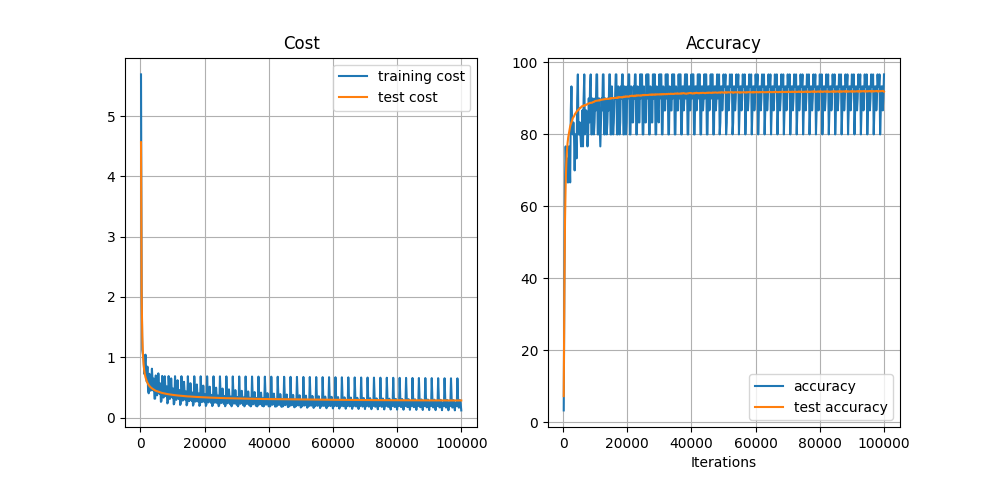
\includegraphics[width=\linewidth]{figures/training_1layer.png}
  \caption{Training history, model 1}
  \label{fig:img1}
\end{minipage}
\begin{minipage}{0.5\textwidth}
  \centering
  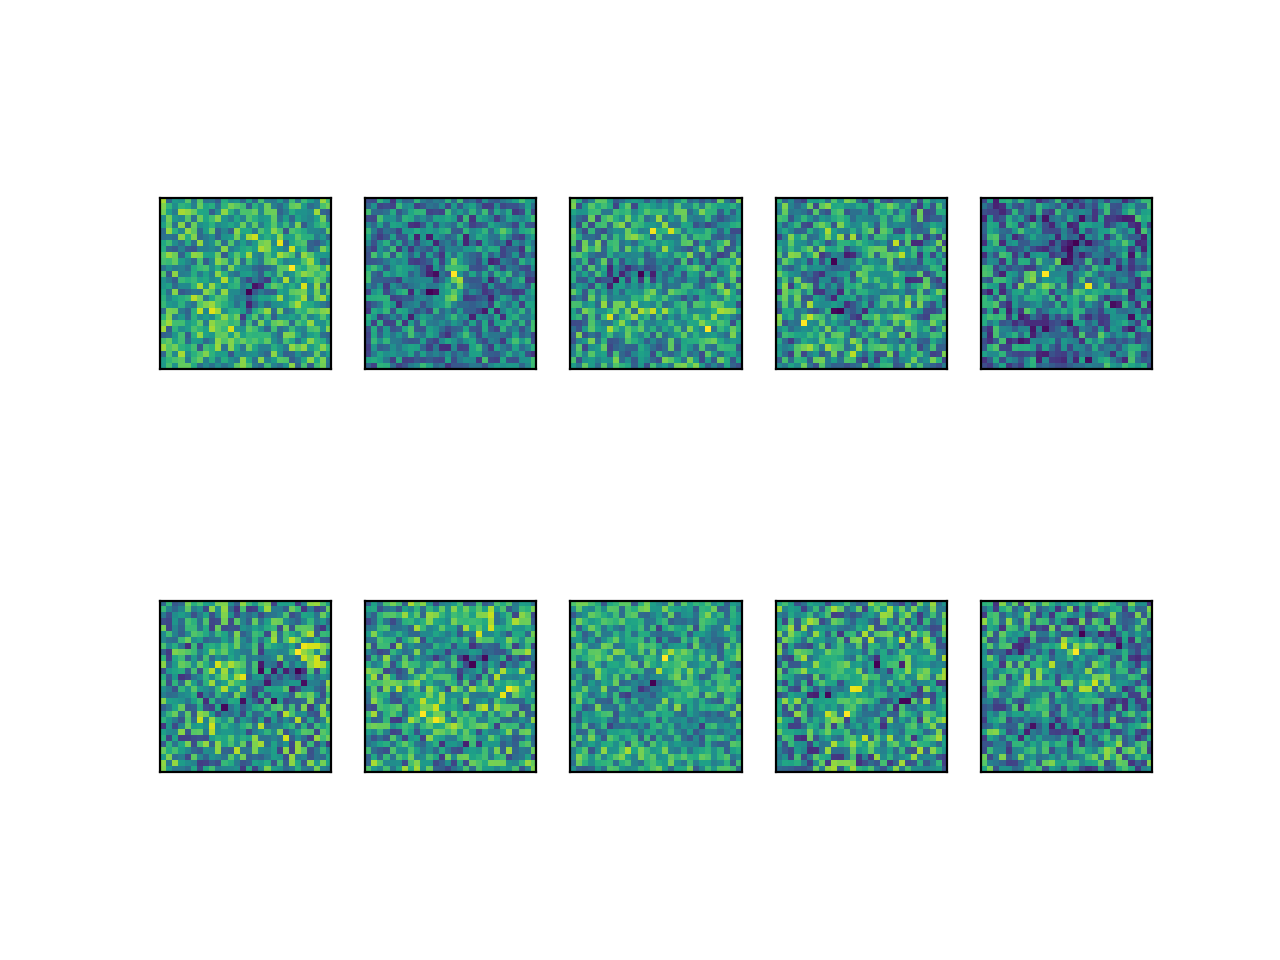
\includegraphics[width=\linewidth]{figures/Figure_1.png}
  \caption{Reshaped weight matrix, model 1}
  \label{fig:img2}
\end{minipage}
\end{figure}


\begin{figure}[h]
\begin{minipage}{0.5\textwidth}
  \centering
  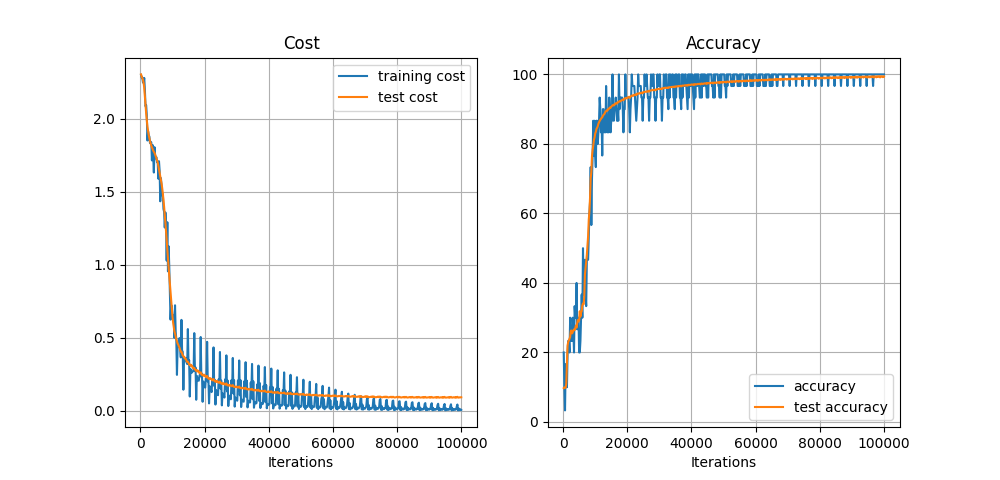
\includegraphics[width=\linewidth]{figures/training_3layer.png}
  \caption{Training history, model 2}
  \label{fig:img1}
\end{minipage}
\begin{minipage}{0.5\textwidth}
  \centering
  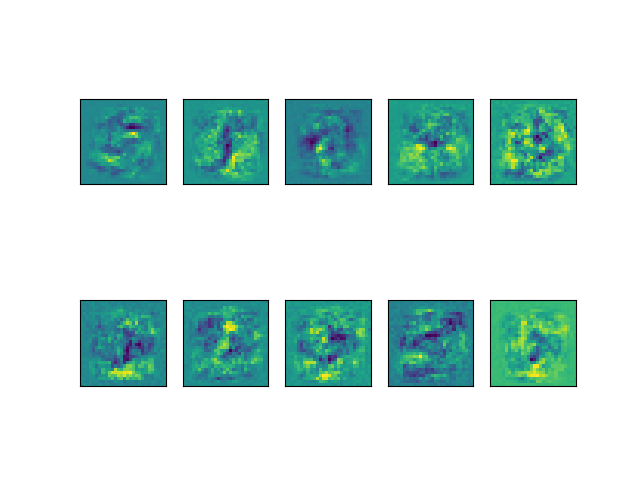
\includegraphics[width=\linewidth]{figures/Figure_2.png}
  \caption{Reshaped weight matrix, model 2}
  \label{fig:img2}
\end{minipage}
\end{figure}


We can see that the case of the one layer network, the network is not complex enough when the train accuracy never get close to 100\% accuracy even though the batch size was really small, 30 images in each batch. In model with three layers we can see that the gap between the cost for training and test starts to open up that can indicate over training. We also see that the network is complex enough as the training accuracy can hit 100\% with this batch size (30 images). The model with the Sigmoid activation function was much harder to train and suffered a bit from the initialization not being optimal for this activation function. This lead to slow learning and poor accuracy.

Taking a look on the images of the weight we can see in the one layer model (if we squint with our eyes a bit) that they resemble the digits: 0, 1, 2 and 3. The rest of them are harder to see. This is not so surprising since we try to achieve a high softmax score for the correct digit, by taking the dot product with a similar digit will result in a mean value of the matrix. Quite similar to using the singular value decomposition method to classify the MNIST data set. In the case with the multilayer models it is harder to make out of how the model have tuned the weights since there are multiple layers after with each other.   


\begin{thebibliography}{1}

\bibitem{Asimov} Asimov, Issac (1942). Runaround

\end{thebibliography}

\end{document}
